%%%%%%%%%%%%%%%%%%%%%%%%%%%%%%%%%%%%%%%%%%%%%%%%%%%
%
%  New template code for TAMU Theses and Dissertations starting Fall 2016.  
%
%
%  Author: Sean Zachary Roberson
%  Version 3.17.09
%  Last Updated: 9/21/2017
%
%%%%%%%%%%%%%%%%%%%%%%%%%%%%%%%%%%%%%%%%%%%%%%%%%%%
%%%%%%%%%%%%%%%%%%%%%%%%%%%%%%%%%%%%%%%%%%%%%%%%%%%%%%%%%%%%%%%%%%%%%%
%%                           SECTION III
%%%%%%%%%%%%%%%%%%%%%%%%%%%%%%%%%%%%%%%%%%%%%%%%%%%%%%%%%%%%%%%%%%%%%

\chapter{UNSTRUCTURED MESHING AND LOAD BALANCING IN PDT}\label{cha:lb}

Initially, PDT only swept on structured, logically Cartesian meshes. As the need to solve problems with more complex geometries arose, PDT added a support for arbitrary polyhedral unstructured meshes. However, this introduced imbalanced partitions (or different amounts of cells per processor), causing longer and unmanageable runtimes.

To combat imbalanced partitions, two load balancing algorithms were implemented, referred to in this thesis as the original load-balancing algorithm \cite{mastersthesis,mc2017} and the load-balancing-by-dimension algorithm.

Before detailing the two load balancing algorithms PDT employs, a quick review of partitioning unstructured meshes in PDT is necessary:
\begin{itemize}
\item ``Cut lines'' in 2D (``cut planes'' in 3D) are used to slice through the mesh in the $x$, $y$, and $z$ dimensions.
\item The cut planes form brick partitions, called subsets, that have unstructured meshes inside of them. 
\item Discontinuities along subset boundaries are fixed by ``stitching'' hanging nodes, creating degenerate polygons along subset boundaries.
\item The subsets are distributed amongst the processor domain.
\end{itemize}
Using cut lines/cut planes to partition unstructured meshes preserved the provably optimal sweep partitioning \cite{mpadams2013,mpadams2015} of logically Cartesian grids. 
Subsets, rather than the cells, have $(i,j,k)$ indices and will become the base unit when aggregating spatial parameters. That is, $A_x$ and $A_y$ will now represent the number of subsets in $x$ and $y$ aggregated into a task. 
Figure \ref{partitioning_example} shows an example of an unstructured mesh partitioned into 100 subsets in PDT. 
\begin{figure}[H]
\centering
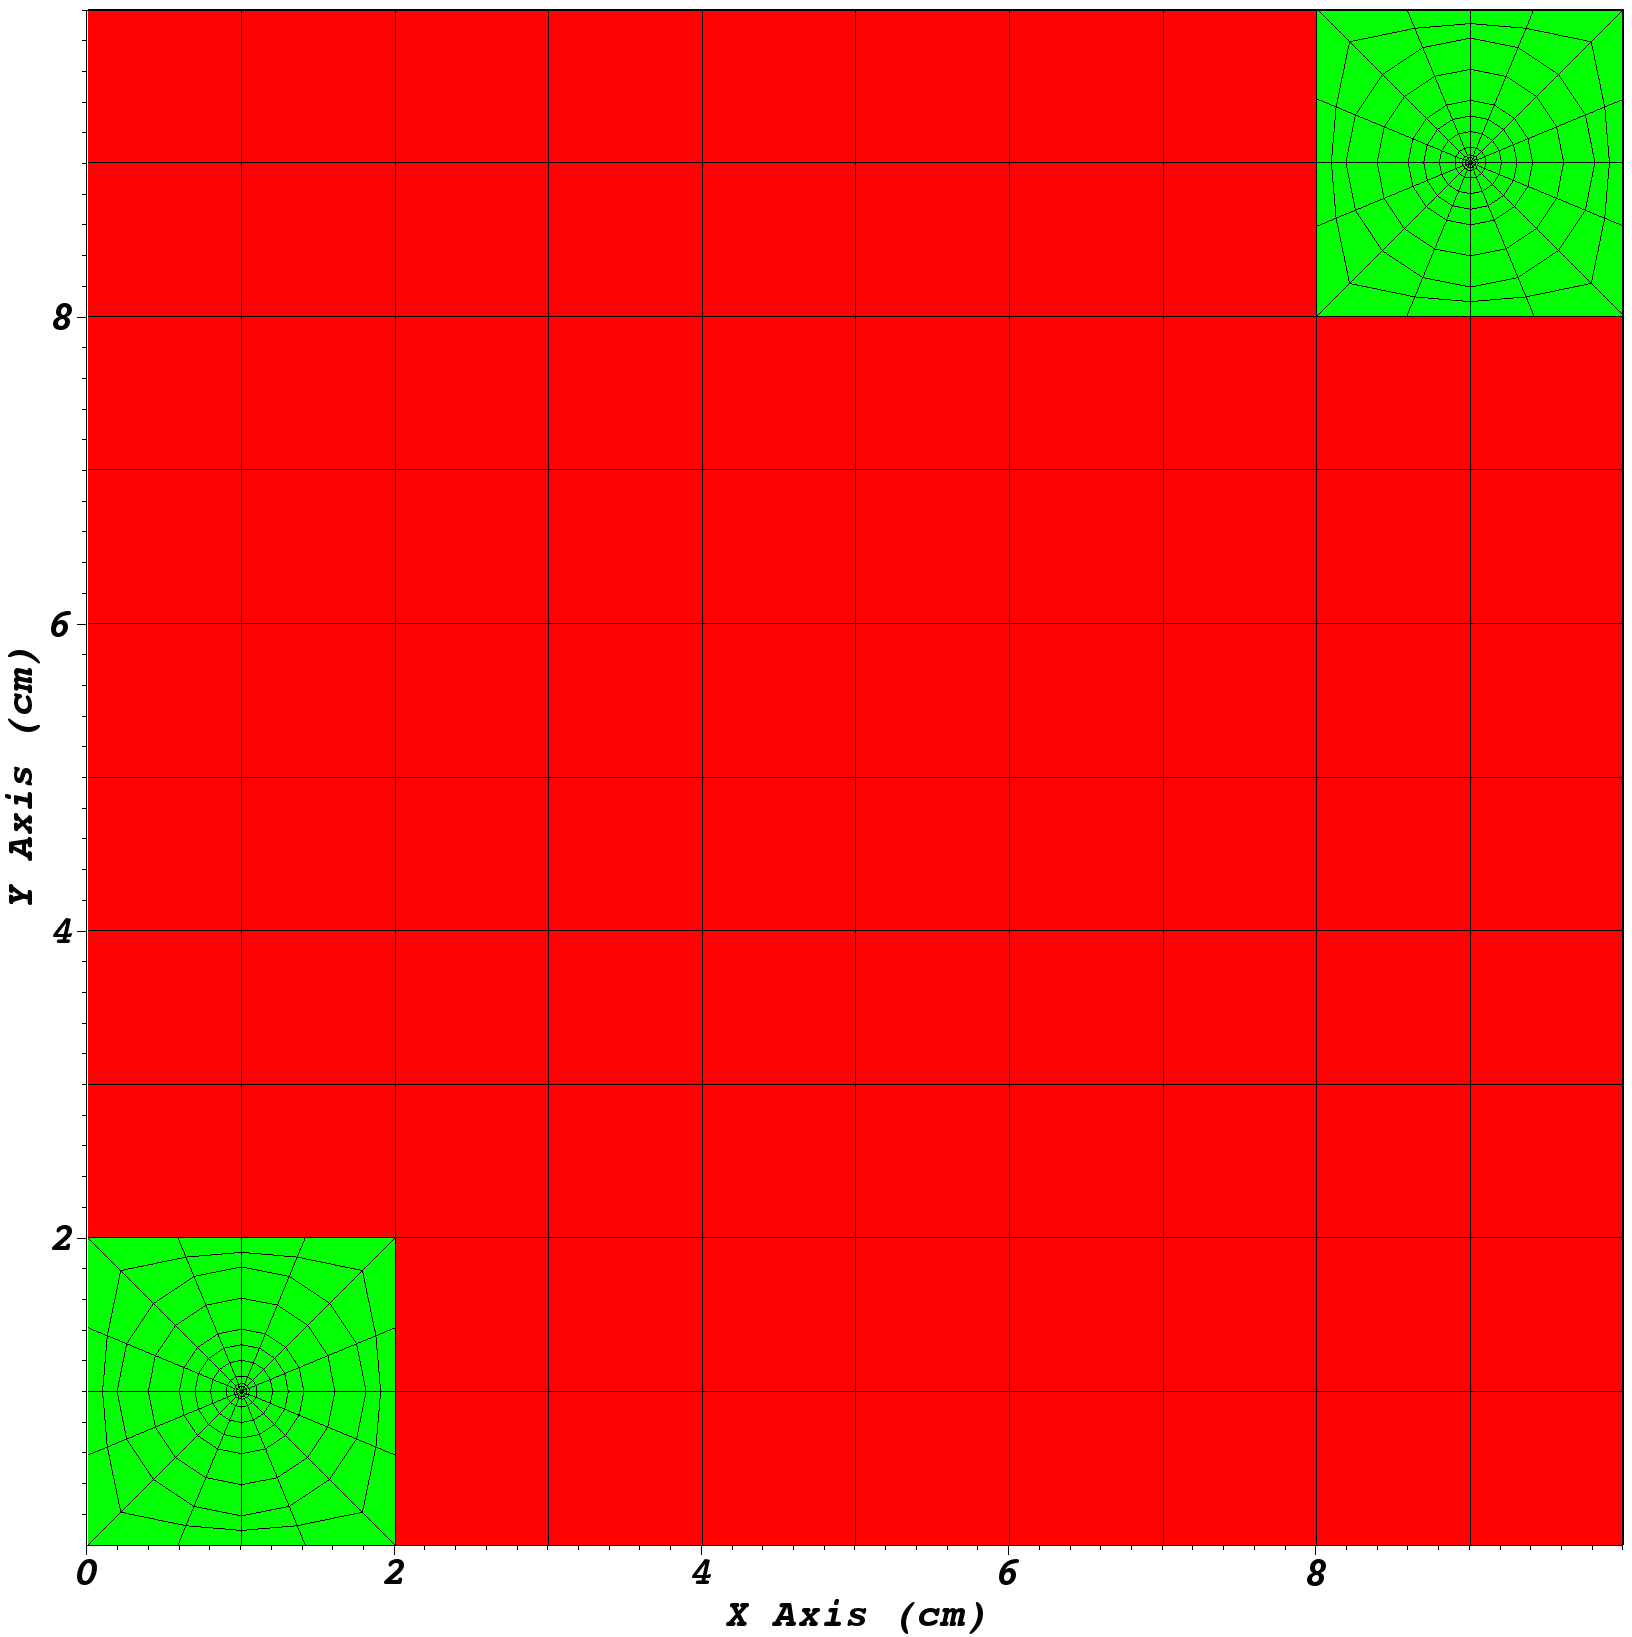
\includegraphics[scale=0.2]{../figures/spiderweb_10x10_sparse.png}
\caption{An unstructured mesh partitioned into 100 subsets with cut lines at 1 cm intervals in both dimensions}
\label{partitioning_example}
\end{figure}

Upon creation, the subsets may have geometric discontinuities as a result of slicing through the mesh. 
Figure \ref{hanging_node} shows an example of a hanging node across a subset boundary. 
This node is stitched across the boundary to preserve geometric continuity, forming a degenerate polygon \cite{degenerate} (in Fig. \ref{hanging_node}, a degenerate square). 
PDT uses Piece-Wise Linear Discontinuous (PWLD) finite-element basis functions \cite{pwld_ragusa,pwld_teresa} that allow for solutions on arbitrary and degenerate polyhedra. 
\begin{figure}[H]
  \centering
  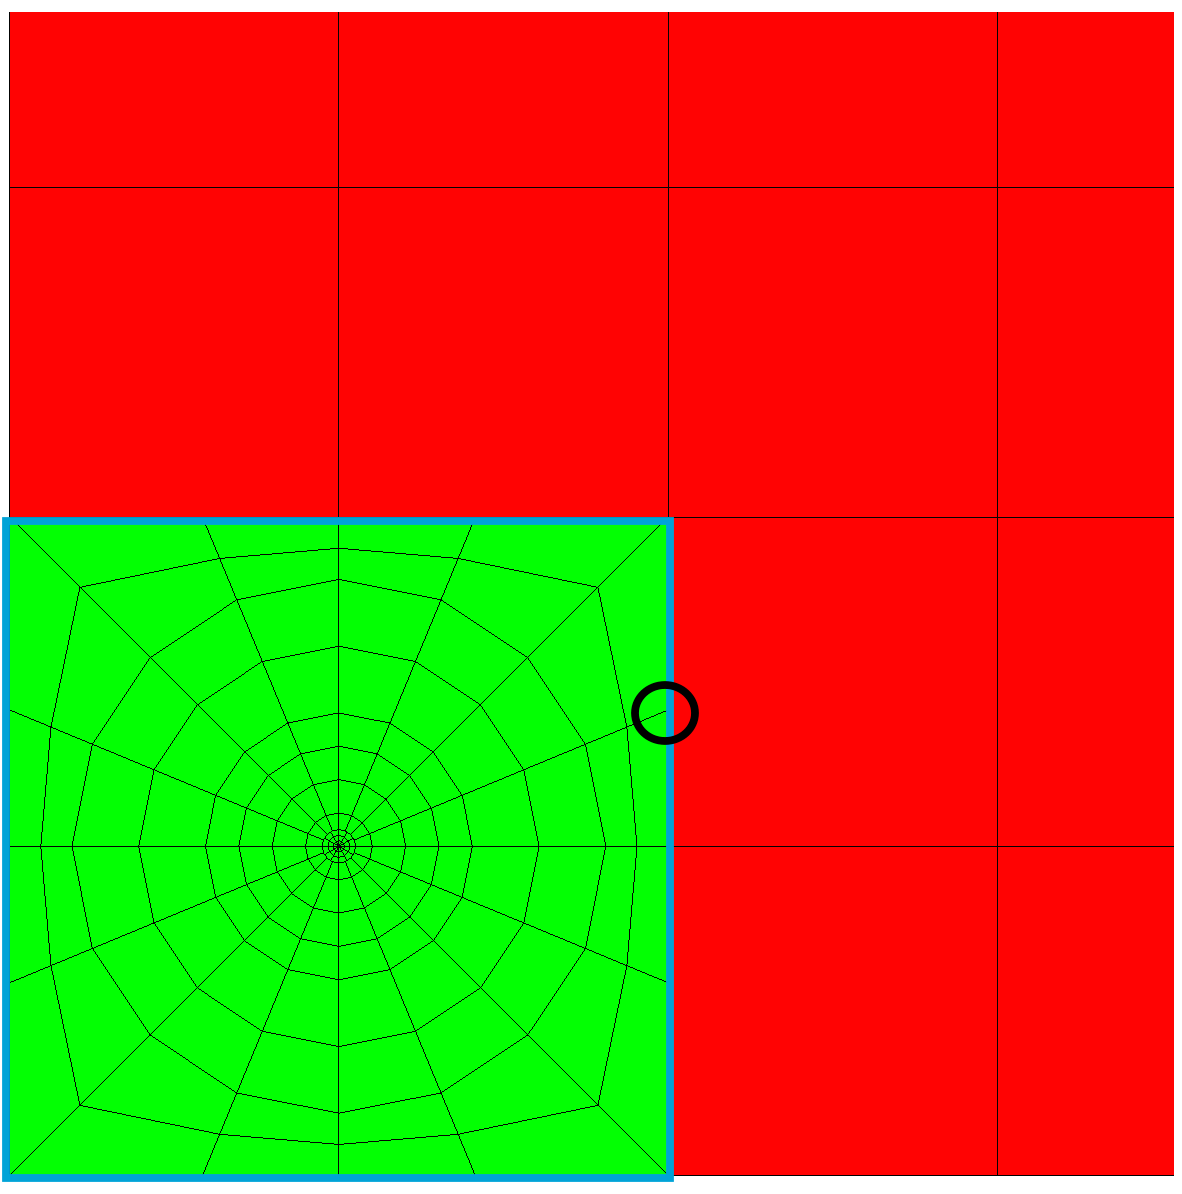
\includegraphics[scale=0.2]{../../figures/hanging_node_spiderweb_example.png}
   \caption{A hanging node (circled in black) on a subset boundary (highlighted in blue).}
   \label{hanging_node}
\end{figure}

Both approaches to load balancing move cut lines in order to redistribute cells more evenly throughout subsets. We define a metric describing how imbalanced our problem is:
\begin{equation}
f =\frac{\underset{ijk}{\text{max}}(N_{ijk})}{\frac{N_{tot}}{I\cdot J\cdot K}},
\label{metric_def}
\end{equation}
where $f$ is the load balance metric, $N_{ijk}$ is the number of cells in subset $(i,j,k)$, $N_{tot}$ is the global number of cells in the problem, and $I$, $J$, and $K$ are the total number of subsets in the $x$, $y$, and $z$ directions, respectively. The metric is a measure of the maximum number of cells per subset divided by the average number of cells per subset. For a perfectly balanced problem, $f = 1$.

Figure \ref{redistribute} illustrates an example of redistributing the cut planes in $x$ to balance the cells per column.
\begin{figure}[H]
\centering
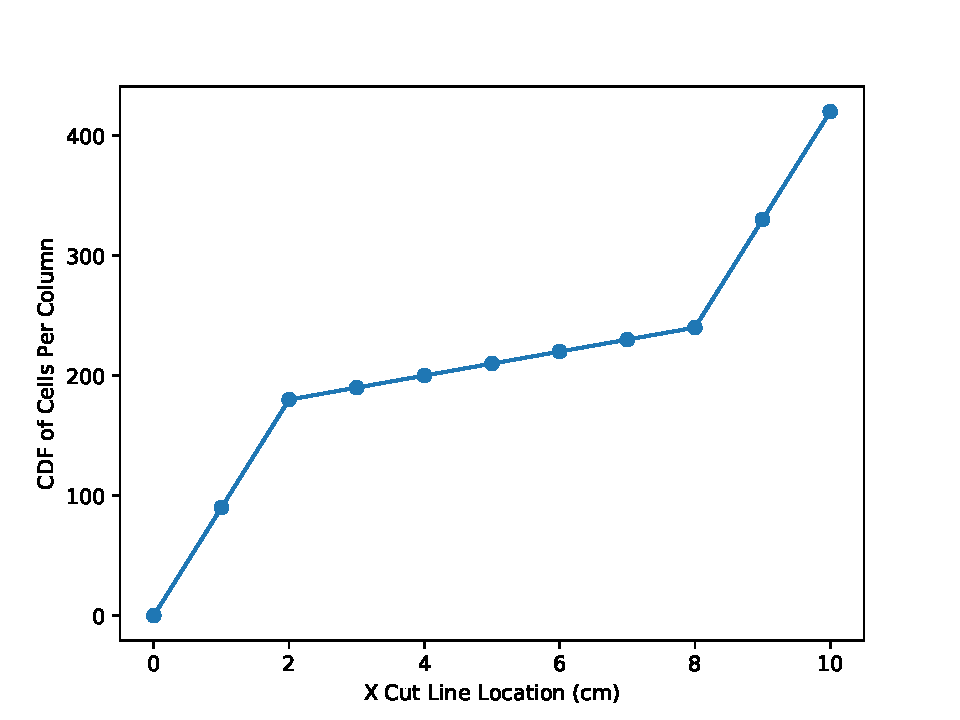
\includegraphics[scale=0.4]{../figures/spiderweb_redistribute_before_sparse.pdf}
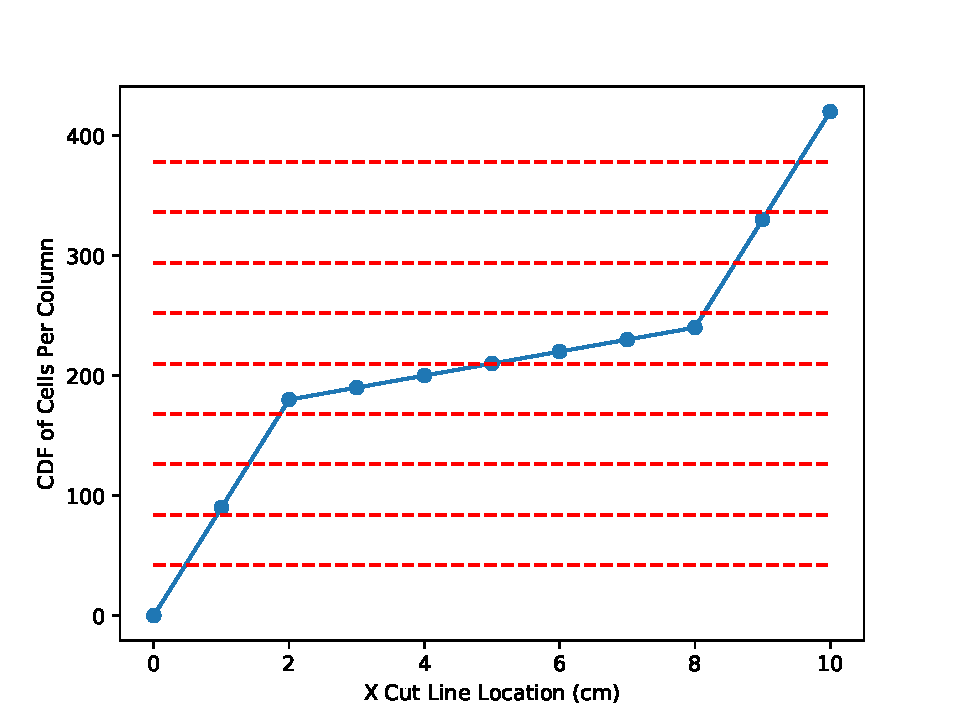
\includegraphics[scale=0.4]{../figures/spiderweb_redistribute_after_sparse.pdf}
\caption{The use of the CDF of cells per column to redistribute the cut lines in X.}
\label{redistribute}
\end{figure}
The image on the left side of Fig. \ref{redistribute} shows the CDF of the cells per column in Fig. \ref{partitioning_example}. The red lines on the right side of Fig. \ref{redistribute} show the ideal equal number of cells per column. The x-value of the intersection of these red lines and the CDF are where the cut lines are redistributed to. 

In order to decide the necessity of redistributing a dimension's cut lines/planes, we use dimensional sub-metrics of the following form:
\begin{equation}
f_{Z} = \frac{\underset{k}{\text{max}}[\sum_{i,j} N_{ijk}]}{\frac{N_{tot}}{K}},
\label{f_z}
\end{equation}
where $K$ is the total number of z-planes. 
Equation \ref{f_z} is a metric defining how imbalanced the problem's planes are. It calculates the maximum cells per plane divided by the average cells per plane. If $f_K$ is greater than a predefined tolerance, the z cut planes are redistributed using the process in Fig. \ref{redistribute}. 
 
\section{Original Load-Balancing Algorithm}
\label{sec:og_lb}

The initial approach to load balancing was implemented on 2D extruded meshes, meaning the mesh is balanced in the 2D plane and then extruded, yielding a balanced 3D mesh. The metrics for this algorithm are defined as follows:
\begin{align}
f &= \frac{\underset{ij}{\text{max}}(N_{ij})}{\frac{N_{tot}}{I\cdot J}}  \label{og_metric}\\
f_X &= \frac{\underset{i}{\text{max}}[\sum_{j} N_{ij}] } {\frac{N_{tot}}{I}} \label{og_i_metric} \\
f_Y &= \frac{\underset{j}{\text{max}}[\sum_{i} N_{ij}] } {\frac{N_{tot}}{J}} \label{og_j_metric}
\end{align}
Equation \ref{og_metric} mirrors Eq. \ref{metric_def} for 2 dimensions, and Eqs. \ref{og_i_metric} and \ref{og_j_metric} define the column and row-wise metrics respectively. 

 Algorithm \ref{initial_algorithm} summarizes the original approach to load balancing meshes in PDT.
\begin{algorithm}[H]
\caption{The original load-balancing algorithm.}
\label{initial_algorithm}
\begin{algorithmic}

\WHILE{$f > 1 + \text{tol}_{\text{subset}}$}
  \IF {$f_X > 1 + \text{tol}_{\text{col}}$}
    \STATE Redistribute the X cut lines.
  \ENDIF
  \IF {$f_Y > 1 + \text{tol}_{\text{row}}$}
  	\STATE Redistribute the Y cut lines.
  \ENDIF
\ENDWHILE
\end{algorithmic}
\end{algorithm}
While the problem is not balanced:
\begin{itemize}
  \item Check if the columns are balanced, and if not redistribute the X cut lines.
  \item Check if the rows are balanced, and if not redistribute the Y cut lines.
  \item Repeat until the mesh is balanced or until a maximum number of iterations is reached.
\end{itemize}

The original load-balancing algorithm placed cut lines in all dimensions all the way through the mesh. 
This created an orthogonal partitioning where each subset had an equivalent number of neighbors, which was done to preserve the provably optimal sweep partitioning described by Adams et. al \cite{mpadams2013,mpadams2015}. 
However, there are theoretical limits to load balancing in this fashion. Figure \ref{2dgeneral} shows a simple 2D subset layout with $M$ unaligned patches with $N$ cells each.

\begin{figure}[H]
\centering
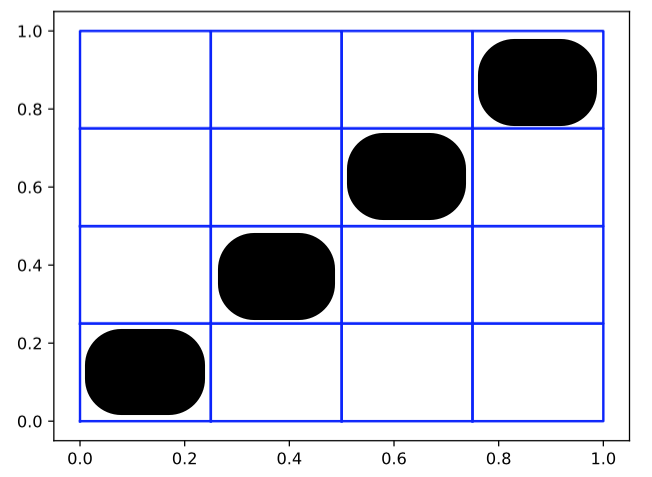
\includegraphics[scale=0.4]{../figures/theoretical_plot.png}
 \caption{A 2D subset layout with $M$ unaligned patches of high mesh density $N$.}
\label{2dgeneral}
\end{figure}
The subset layout is $M^2$, but only $M$ subset have significant work, leading to a theoretical limit for the load imbalance factor:
\begin{equation}
f= \frac{N}{(MN+C)/M^2} \xrightarrow{N\to \infty} \frac{N}{N/M} = M.
\end{equation}
Due to this theoretical limit, the load-balancing-by-dimension algorithm was developed.

\section{Load-Balancing-by-Dimension Algorithm}
\label{sec:lbd}

The load-balancing-by-dimension by dimension (LBD) algorithm, similar to the original load-balancing algorithm, relies on the movement of cut lines/planes to redistribute mesh cells in a more balanced manner.
However, cut lines are no longer required to go all the way through the mesh, and the load-balancing-by-dimension algorithm is fully extensible to 3 dimensions. 
The load-balancing-by-dimension algorithm is summarized by:
\begin{enumerate}
  \item Slice the mesh in $z$ and redistribute cut planes until each plane has approximately an equivalent number of cells.
  \item For each $z$ layer, slice the layer in columns and redistribute the $x$ cut lines until each column has an approximately equivalent number of cells.
  \item For each column within each $z$ layer, slice the column in rows and redistribute the $y$ cut lines until each row has an approximately equivalent number of cells.
\end{enumerate}

We once again use dimensional sub-metrics to determine whether or not a dimension's cut lines/planes need to be redistributed. The $z$ dimension's sub-metric is defined by Eq. \ref{f_z}. For the LBD algorithm, there are $K$ column-wise metrics, one for each $z$ layer:
\begin{equation}
f_{X,k} = \frac{ \underset{i}{\text{max}}[ \sum_{j} N_{ijk}]  }  {\frac{N_{tot,k}}{I}}.
\label{lbd_x_metric}
\end{equation}
Equation \ref{lbd_x_metric} defines the column-wise metric for layer $k$, or the maximum number of cells per column in layer $k$ divided by the average number of cells per column in layer $k$. 

For the LBD algorithm, there are $K\cdot I$ row-wise metrics, one for each column in each $z$ layer:
\begin{equation}
f_{Y,k,i} = \frac{\underset{j}{\text{max}} N_{ijk} } {\frac{N_{tot,k,i}}{J}}.
\label{lbd_y_metric}
\end{equation}
Equation \ref{lbd_y_metric} defines the row-wise metric for layer $k$ in column $i$, or the maximum number of cells per row in column $i$ in layer $k$ divided by the average number of cells per row in column $i$ in layer $k$. 

Algorithm \ref{lbd} details the load-balancing-by-dimension algorithm. 
\begin{algorithm}[H]
\caption{The load-balancing-by-dimension algorithm.}
\label{lbd}
\begin{algorithmic}

  \WHILE {$f_{Z} > 1 + \text{tol}_{\text{K}}$}
    \STATE Redistribute the Z cut planes.
  \ENDWHILE  
  
  \FOR {$k$ in $K$}
    \WHILE {$f_{X,k} > 1 + \text{tol}_{\text{I}}$}
      \STATE Redistribute the X cut lines within layer $k$. 
    \ENDWHILE
  \ENDFOR
  
  \FOR{$k$ in $K$}
    \FOR{$i$ in $I$}
      \WHILE {$f_{Y,k,i} > 1 +  \text{tol}_{\text{J}}$ }
        \STATE Redistribute the Y cut lines in column $i$ in layer $k$. 
      \ENDWHILE
    \ENDFOR
  \ENDFOR
  
  \STATE Calculate $f$.
\end{algorithmic}
\end{algorithm}

Figure \ref{alg_illustration} illustrates the behavior of both algorithms. In the left image of the figure, we see the partitions cutting across the entire domain, with the left-most $x$ cut line moved into the denser geometric feature in the bottom left corner to more evenly distribute cells. In the right image of the figure, we see the $x$ partitions cutting across the entire domain, but the $y$ partitions being redistributed by column. The $y$ partitions are moved into the respective geometric features in the appropriate columns in order to better balance the problem.

\begin{figure}[H]
\centering
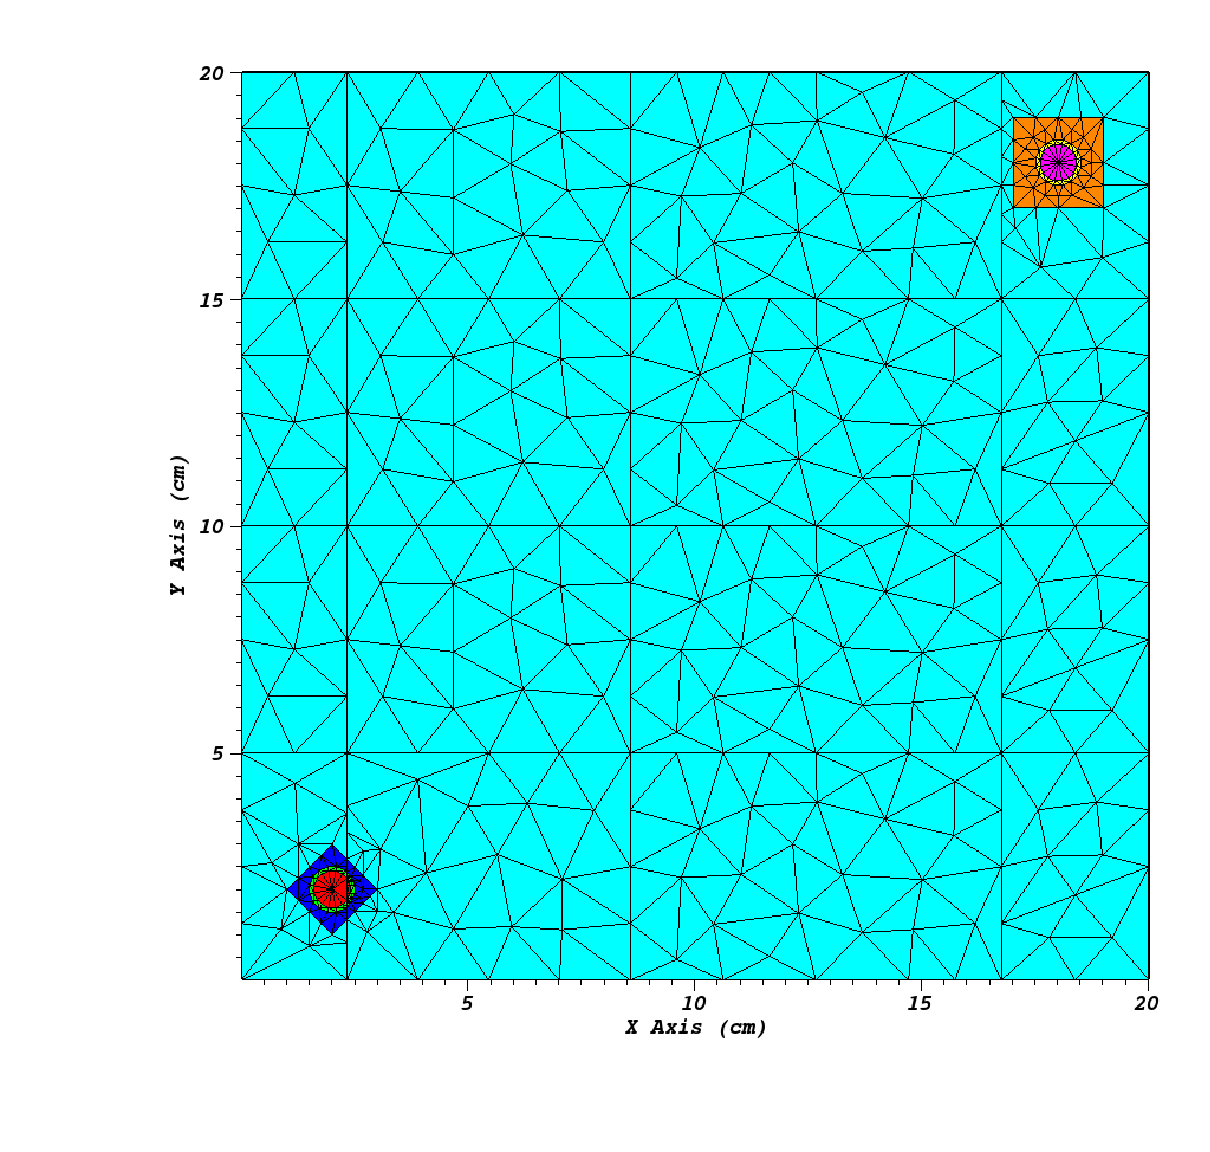
\includegraphics[scale=0.45,trim={0.95in 0.64in 0.35in 0.44in},clip]{../figures/og_lb_example.pdf}
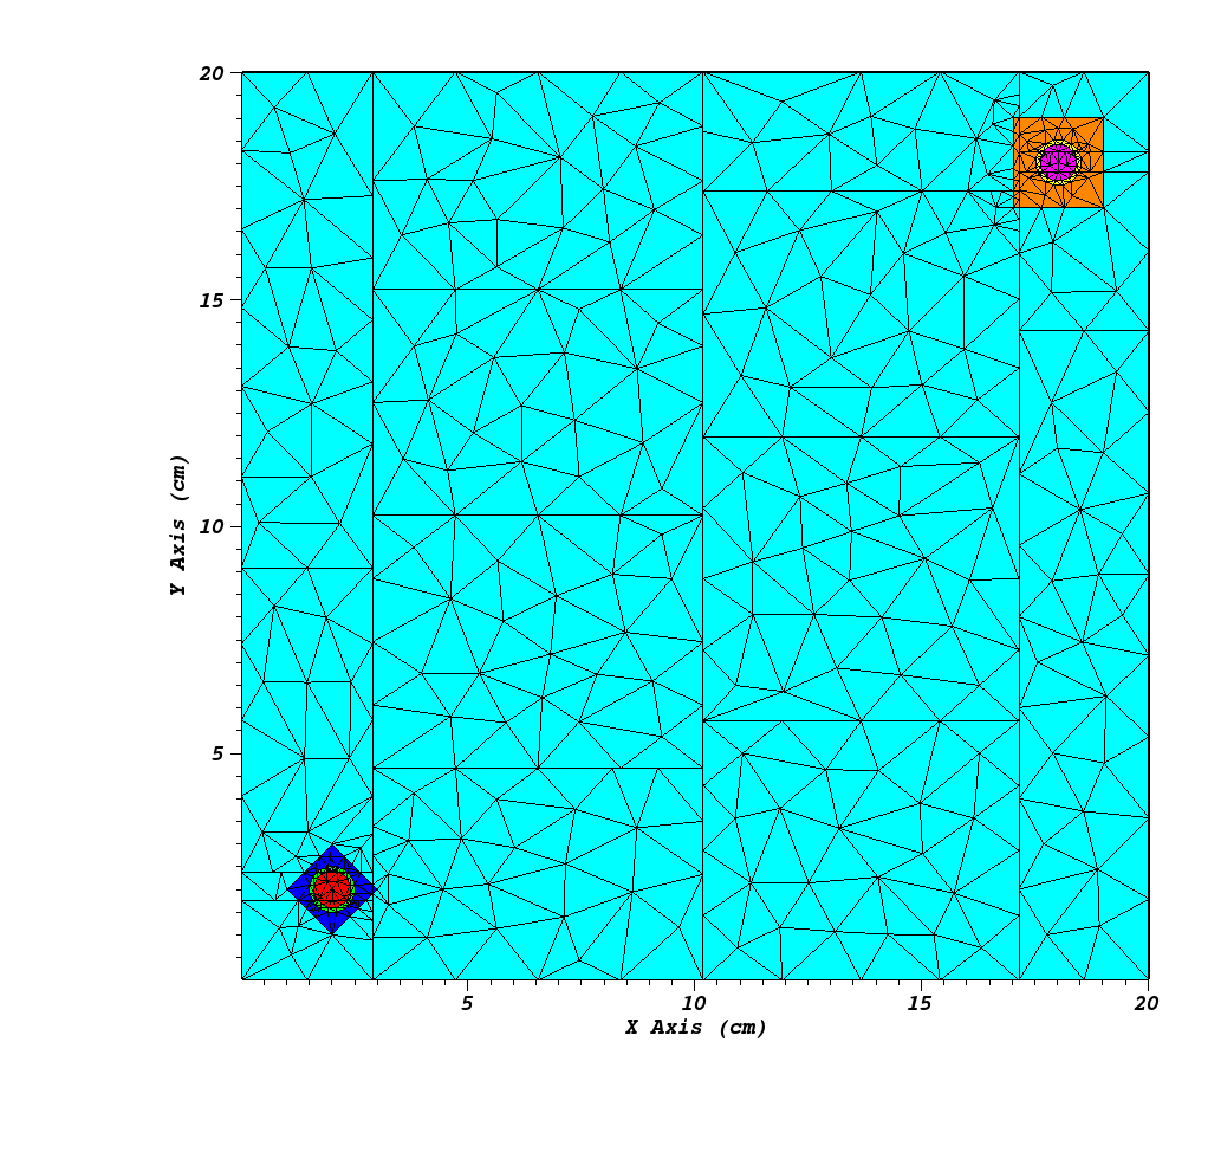
\includegraphics[scale=0.45,trim={0.95in 0.64in 0.35in 0.44in},clip]{../figures/lbd_example.pdf}
\caption{The partitions of a problem after the original load balancing (left) and the load-balancing-by-dimension (right) algorithms.}
\label{alg_illustration}
\end{figure}


\section{Results}

To show the behavior of the original load balancing algorithm and the load-balancing-by-dimension algorithm, the problem shown in Fig. \ref{partitioning_example} was run with a varying number of subsets and with a varying maximum triangle area, with the minimum allowable angle per triangle was kept constant at \ang{20}. We varied the number of subsets in $x$ and $y$ from 2 to 10 (with the total number of subsets varying from 4 to 100). The problem illustrated by Fig. \ref{partitioning_example} was chosen because it has two dense features in opposing corners with no features in between, lending itself to being an imbalanced mesh. Table \ref{og_table} shows the results of this parametric study using the original load balancing algorithm vs. using the load-balancing-by-dimension algorithm. Table \ref{all_improvements} shows the percent improvements for both algorithms from no load balancing to running both load balancing algorithm, while Table \ref{method_improvement} shows the improvement of the load-balancing-by-dimension algorithm relative to the original load balancing algorithm.

%\vspace{-1cm}
\begin{table}[H]
\centering
  \caption{\bf The results of the parametric study using the original load balancing algorithm (left) and the load-balancing-by-dimension algorithm (right).}
  \scalebox{0.5}{
  \begin{tabular}{c|c|c|c|c|c|c|c|c|c} 
  \bf Area, $N^{1/2}$ & \bf  2 &  \bf 3    &  \bf  4   &  \bf  5   &  \bf  6   &  \bf  7   & \bf   8   &  \bf 9    &  \bf 10   \\ \hline \hline
\bf Coarse&1.993 & 2.735 & 4.360 & 4.812 & 5.545 & 6.321 & 3.114 & 2.697 & 1.893 \\ \hline 
\bf 1.8& 1.408 & 2.277 & 2.886 & 3.269 & 4.716 & 4.721 & 5.890 & 4.618 & 1.863 \\ \hline
\bf 1.6& 1.375 & 2.206 & 2.649 & 3.247 & 4.356 & 4.876 & 4.678 & 5.062 & 1.329 \\ \hline
\bf 1.4& 1.337 & 2.110 & 2.982 & 3.031 & 4.615 & 4.310 & 8.911 & 4.652 & 2.675 \\ \hline
\bf 1.2& 1.344 & 2.008 & 2.017 & 3.392 & 3.916 & 4.969 & \cellcolor{blue!25}9.576 & 4.543 & 4.728 \\ \hline
\bf 1.0& 1.264 & 1.806 & 2.405 & 2.976 & 3.657 & 4.317 & 6.242 & 4.831 & 4.941 \\ \hline
\bf 0.8& 1.212 & 1.640 & 2.300 & 2.436 & 2.941 & 4.395 & 7.420 & 4.466 & 3.947 \\ \hline
\bf 0.6& 1.153 & 1.567 & 2.045 & 2.368 & 3.199 & 2.999 & 7.206 & 4.101 & 3.592 \\ \hline
\bf 0.4& 1.108 & 1.411 & 1.633 & 2.117 & 2.383 & 2.646 & 6.970 & 3.086 & 2.511 \\ \hline
\bf 0.2& 1.052 & 1.197 & 1.258 & 1.523 & 1.789 & 1.857 & 3.380 & 2.193 & 1.883 \\ \hline
\bf 0.1& 1.029 & 1.092 & 1.149 & 1.207 & 1.276 & 1.420 & 2.015 & 1.565 & 1.247 \\ \hline
\bf 0.08& 1.009 & 1.043 & 1.086 & 1.101 & 1.179 & 1.267 & 2.118 & 1.551 & 1.271 \\ \hline
\bf 0.06& 1.009 & 1.024 & 1.059 & 1.094 & 1.138 & 1.154 & 1.825 & 1.432 & 1.138 \\ \hline
\bf 0.05& 1.008 & 1.023 & 1.025 & 1.028 & 1.073 & 1.149 & 1.666 & 1.380 & 1.110 \\ \hline
\bf 0.04& 1.005 & 1.016 & 1.017 & 1.021 & 1.038 & 1.051 & 1.520 & 1.311 & 1.080 \\ \hline
\bf 0.03& 1.005 & 1.008 & 1.018 & 1.039 & 1.059 & 1.073 & 1.450 & 1.179 & \cellcolor{red!25}1.001 \\ \hline
\bf 0.02& 1.005 & 1.008 & 1.010 & 1.013 & 1.021 & 1.035 & 1.623 & 1.137 & 1.016 \\ \hline
\bf 0.01& 1.003 & 1.009 & 1.009 & 1.011 & 1.016 & 1.013 & 1.281 & 1.058 & 1.015 \\ \hline
  \end{tabular}}
 \scalebox {0.5}{
   \begin{tabular}{c|c|c|c|c|c|c|c|c|c} 
\bf Area, $N^{1/2}$ & \bf  2 & \bf 3    &  \bf  4   &  \bf  5   &  \bf 6    &  \bf  7   &   \bf 8   &  \bf 9    &  \bf 10   \\ \hline \hline
\bf Coarse & 1.645 & 1.455 & 1.878 & 2.348 & 3.046 & 3.022 & 1.752 & 2.304 & 1.451 \\ \hline 
\bf 1.8& 1.034 & 1.460 & 2.127 & 1.744 & 2.098 & 2.588 & 2.623 & 2.776 & 2.872 \\ \hline
\bf 1.6& 1.015 & 1.396 & 1.899 & 1.877 & 2.090 & 2.857 & 2.608 & 3.582 & 2.604 \\ \hline
\bf 1.4& 1.011 & 1.418 & 1.631 & 1.964 & 1.820 & 2.968 & 2.055 & 2.201 & 1.523 \\ \hline
\bf 1.2& 1.019 & 1.344 & 1.483 & 1.983 & 2.122 & 3.023 & 2.356 & \cellcolor{blue!25}4.765 & 2.371 \\ \hline
\bf 1.0& 1.007 & 1.338 & 1.641 & 2.313 & 3.097 & 2.098 & 2.563 & 2.808 & 2.637 \\ \hline
\bf 0.8& 1.016 & 1.157 & 1.457 & 1.982 & 1.881 & 2.340 & 2.283 & 3.513 & 3.947 \\ \hline
\bf 0.6& 1.012 & 1.111 & 1.199 & 1.598 & 1.901 & 1.791 & 2.330 & 3.005 & 3.719 \\ \hline
\bf 0.4& 1.005 & 1.024 & 1.204 & 1.288 & 1.665 & 1.492 & 1.660 & 2.528 & 2.511 \\ \hline
\bf 0.2& 1.007 & 1.021 & 1.025 & 1.116 & 1.175 & 1.358 & 1.478 & 1.624 & 1.837 \\ \hline
\bf 0.1& 1.003 & 1.019 & 1.024 & 1.019 & 1.092 & 1.122 & 1.161 & 1.087 & 1.247 \\ \hline
\bf 0.08& 1.007 & 1.010 & 1.022 & 1.035 & 1.035 & 1.077 & 1.176 & 1.135 & 1.219 \\ \hline
\bf 0.06& 1.004 & 1.009 & 1.021 & 1.032 & 1.031 & 1.070 & 1.102 & 1.080 & 1.072 \\ \hline
\bf 0.05& 1.002 & 1.005 & 1.019 & 1.023 & 1.038 & 1.071 & 1.096 & 1.094 & 1.101 \\ \hline
\bf 0.04& 1.002 & 1.008 & 1.008 & 1.021 & 1.027 & 1.028 & 1.063 & 1.091 & 1.080 \\ \hline
\bf 0.03& 1.003 & 1.008 & 1.013 & 1.014 & 1.030 & 1.044 & 1.068 & 1.074 & \cellcolor{red!25}1.001 \\ \hline
\bf 0.02& 1.002 & 1.006 & 1.009 & 1.013 & 1.020 & 1.030 & 1.038 & 1.058 & 1.016 \\ \hline
\bf 0.01& \cellcolor{red!25}1.001 & 1.006 & 1.007 & 1.011 & 1.015 & 1.013 & 1.030 & 1.029 & 1.015 \\ \hline

  \end{tabular}} 
  \label{og_table}
\end{table}

\begin{table}[H]
\centering
\caption{\bf The percent improvement of the original load balancing algorithm (left) and the load-balancing-by-dimension algorithm (right).}
\scalebox{0.5}{
\begin{tabular}{c|c|c|c|c|c|c|c|c|c} 

\bf Area, $N^{1/2}$ & \bf  2 & \bf 3    &  \bf  4   &  \bf  5   &  \bf 6    &  \bf  7   &   \bf 8   &  \bf 9    &  \bf 10   \\ \hline \hline
\bf Coarse& 0.000 & 0.367 & 0.403 & 0.552 & 0.628 & 0.491 & 0.890 & 0.720 & 0.765 \\ \hline 
 \bf 1.8& 0.000 & 0.091 & 0.337 & 0.364 & 0.473 & 0.390 & 0.767 & 0.413 & 0.683 \\ \hline 
 \bf 1.6& 0.000 & 0.093 & 0.398 & 0.368 & 0.499 & 0.370 & 0.815 & 0.353 & 0.774 \\ \hline 
 \bf 1.4& 0.000 & 0.061 & 0.080 & 0.410 & 0.415 & 0.412 & 0.570 & 0.413 & 0.545 \\ \hline 
 \bf 1.2& 0.000 & 0.007 & 0.391 & 0.340 & 0.378 & 0.315 & 0.536 & 0.245 & 0.196 \\ \hline 
 \bf 1.0& 0.000 & 0.038 & 0.206 & 0.420 & 0.341 & 0.186 & 0.696 & 0.201 & 0.160 \\ \hline 
 \bf 0.8& 0.000 & 0.049 & 0.109 & 0.336 & 0.434 & 0.139 & 0.637 & 0.228 & 0.000 \\ \hline 
 \bf 0.6& 0.000 & 0.000 & 0.057 & 0.199 & 0.163 & 0.346 & 0.517 & 0.000 & 0.090 \\ \hline 
 \bf 0.4& 0.000 & 0.000 & 0.065 & 0.013 & 0.267 & 0.147 & 0.528 & 0.179 & 0.000 \\ \hline 
 \bf 0.2& 0.000 & 0.000 & 0.000 & 0.000 & 0.001 & 0.041 & 0.566 & 0.121 & 0.000 \\ \hline 
 \bf 0.1& 0.000 & 0.000 & 0.000 & 0.000 & 0.000 & 0.000 & 0.540 & 0.089 & 0.000 \\ \hline 
 \bf 0.08&0.000 & 0.000 & 0.000 & 0.000 & 0.000 & 0.000 & 0.458 & 0.000 & 0.000 \\ \hline 
 \bf 0.06&0.000 & 0.000 & 0.000 & 0.000 & 0.000 & 0.000 & 0.409 & 0.000 & 0.000 \\ \hline 
 \bf 0.05&0.000 & 0.000 & 0.000 & 0.000 & 0.000 & 0.000 & 0.360 & 0.000 & 0.000 \\ \hline 
 \bf 0.04&0.000 & 0.000 & 0.000 & 0.000 & 0.000 & 0.000 & 0.348 & 0.000 & 0.000 \\ \hline 
 \bf 0.03&0.000 & 0.000 & 0.000 & 0.000 & 0.000 & 0.000 & 0.293 & 0.000 & 0.000 \\ \hline 
 \bf 0.02&0.000 & 0.000 & 0.000 & 0.000 & 0.000 & 0.000 & 0.000 & 0.000 & 0.000 \\ \hline 
 \bf 0.01&0.000 & 0.000 & 0.000 & 0.000 & 0.000 & 0.000 & 0.000 & 0.000 & 0.000 \\ \hline 
\end{tabular}}
\scalebox{0.5}{
\begin{tabular}{c|c|c|c|c|c|c|c|c|c} 
\bf Area, $N^{1/2}$ & \bf  2 & \bf 3    &  \bf  4   &  \bf  5   &  \bf 6    &  \bf  7   &   \bf 8   &  \bf 9    &  \bf 10   \\ \hline \hline
\bf Coarse& 0.175 & 0.663 & 0.743 & 0.781 & 0.796 & 0.757 & 0.938 & 0.760 & 0.820 \\ \hline 
  \bf 1.8& 0.266 & 0.417 & 0.511 & 0.661 & 0.766 & 0.665 & 0.896 & 0.647 & 0.512 \\ \hline 
  \bf 1.6& 0.262 & 0.426 & 0.568 & 0.635 & 0.760 & 0.631 & 0.897 & 0.542 & 0.557 \\ \hline 
  \bf 1.4& 0.244 & 0.369 & 0.497 & 0.618 & 0.769 & 0.595 & 0.901 & 0.722 & 0.741 \\ \hline 
  \bf 1.2& 0.242 & 0.336 & 0.552 & 0.614 & 0.663 & 0.583 & 0.886 & 0.208 & 0.597 \\ \hline 
  \bf 1.0& 0.203 & 0.287 & 0.458 & 0.549 & 0.442 & 0.605 & 0.875 & 0.536 & 0.552 \\ \hline 
  \bf 0.8& 0.162 & 0.330 & 0.435 & 0.460 & 0.638 & 0.542 & 0.888 & 0.393 & 0.000 \\ \hline 
  \bf 0.6& 0.122 & 0.291 & 0.447 & 0.460 & 0.503 & 0.610 & 0.844 & 0.267 & 0.058 \\ \hline 
  \bf 0.4& 0.093 & 0.274 & 0.310 & 0.400 & 0.488 & 0.519 & 0.888 & 0.328 & 0.000 \\ \hline 
  \bf 0.2& 0.042 & 0.147 & 0.185 & 0.267 & 0.344 & 0.299 & 0.810 & 0.349 & 0.025 \\ \hline 
  \bf 0.1& 0.026 & 0.067 & 0.109 & 0.156 & 0.144 & 0.210 & 0.735 & 0.367 & 0.000 \\ \hline 
  \bf 0.08&0.002 & 0.032 & 0.059 & 0.060 & 0.122 & 0.150 & 0.699 & 0.268 & 0.041 \\ \hline 
  \bf 0.06&0.005 & 0.014 & 0.036 & 0.057 & 0.094 & 0.073 & 0.643 & 0.246 & 0.058 \\ \hline 
  \bf 0.05&0.006 & 0.017 & 0.006 & 0.005 & 0.033 & 0.068 & 0.579 & 0.208 & 0.008 \\ \hline 
  \bf 0.04&0.002 & 0.008 & 0.009 & 0.000 & 0.011 & 0.022 & 0.544 & 0.168 & 0.000 \\ \hline 
  \bf 0.03&0.002 & 0.000 & 0.005 & 0.024 & 0.028 & 0.027 & 0.479 & 0.089 & 0.000 \\ \hline 
  \bf 0.02&0.003 & 0.002 & 0.001 & 0.000 & 0.001 & 0.004 & 0.361 & 0.070 & 0.000 \\ \hline 
  \bf 0.01&0.002 & 0.003 & 0.002 & 0.000 & 0.001 & 0.000 & 0.196 & 0.027 & 0.000 \\ \hline 

\end{tabular}}
\label{all_improvements}
\end{table}

The data in Tables \ref{og_table} and \ref{all_improvements} showcase an important point. As mesh refinement increases, the need for load balancing decreases. If sparse regions of the domain have a similar number of cells to the dense regions of the domain, the problem will be inherently balanced with even partitions. Table \ref{method_improvement} demonstrates that with the exception of a few outliers, the load balancing by dimension algorithm is an improvement over the original load balancing algorithms, particularly for coarser mesh refinements. The metric improves by a max of 76.9\% and a mean of 21.7\%  with the load balancing by dimensions algorithm over the original load balancing algorithm.

%method improvement table
\begin{table}[H]
\centering
\caption{\bf The percent improvement of the load balancing by dimension algorithm over the original load balancing algorithm.}
\scalebox{0.5}{
\begin{tabular}{c|c|c|c|c|c|c|c|c|c} 
\bf Area, $N^{1/2}$ & \bf  2 & \bf 3    &  \bf  4   &  \bf  5   &  \bf 6    &  \bf  7   &   \bf 8   &  \bf 9    &  \bf 10   \\ \hline \hline
Coarse & 0.175 & 0.468 & 0.569 & 0.512 & 0.451 & 0.522 & 0.437 & 0.146 & 0.234 \\ \hline 
 \bf 1.8& 0.266 & 0.359 & 0.263 & 0.466 & 0.555 & 0.452 & 0.555 & 0.399 & -0.542 \\ \hline 
 \bf 1.6& 0.262 & 0.367 & 0.283 & 0.422 & 0.520 & 0.414 & 0.443 & 0.292 & -0.959 \\ \hline 
 \bf 1.4& 0.244 & 0.328 & 0.453 & 0.352 & 0.606 & 0.311 & 0.769 & 0.527 & 0.431 \\ \hline 
 \bf 1.2& 0.242 & 0.331 & 0.265 & 0.415 & 0.458 & 0.392 & 0.754 & -0.049 & 0.499 \\ \hline 
 \bf 1.0& 0.203 & 0.259 & 0.318 & 0.223 & 0.153 & 0.514 & 0.589 & 0.419 & 0.466 \\ \hline 
 \bf 0.8& 0.162 & 0.295 & 0.366 & 0.186 & 0.360 & 0.467 & 0.692 & 0.213 & -0.000 \\ \hline 
 \bf 0.6& 0.122 & 0.291 & 0.414 & 0.325 & 0.406 & 0.403 & 0.677 & 0.267 & -0.035 \\ \hline 
 \bf 0.4& 0.093 & 0.274 & 0.262 & 0.392 & 0.301 & 0.436 & 0.762 & 0.181 & 0.000 \\ \hline 
 \bf 0.2& 0.042 & 0.147 & 0.185 & 0.267 & 0.343 & 0.269 & 0.563 & 0.260 & 0.025 \\ \hline 
 \bf 0.1& 0.026 & 0.067 & 0.109 & 0.156 & 0.144 & 0.210 & 0.424 & 0.305 & -0.000 \\ \hline 
 \bf 0.08&0.002 & 0.032 & 0.059 & 0.060 & 0.122 & 0.150 & 0.445 & 0.268 & 0.041 \\ \hline 
 \bf 0.06&0.005 & 0.014 & 0.036 & 0.057 & 0.094 & 0.073 & 0.396 & 0.246 & 0.058 \\ \hline 
 \bf 0.05&0.006 & 0.017 & 0.006 & 0.005 & 0.033 & 0.068 & 0.342 & 0.208 & 0.008 \\ \hline 
 \bf 0.04&0.002 & 0.008 & 0.009 & 0.000 & 0.011 & 0.022 & 0.301 & 0.168 & -0.000 \\ \hline 
 \bf 0.03&0.002 & -0.000 & 0.005 & 0.024 & 0.028 & 0.027 & 0.263 & 0.089 & 0.000 \\ \hline 
 \bf 0.02&0.003 & 0.002 & 0.001 & 0.000 & 0.001 & 0.004 & 0.361 & 0.070 & 0.000 \\ \hline 
 \bf 0.01&0.002 & 0.003 & 0.002 & -0.000 & 0.001 & -0.000 & 0.196 & 0.027 & -0.000 \\ \hline 
\end{tabular}}
\label{method_improvement}
\end{table}
